\subsection{Diagrama del Modelo Físico}
La Figura \ref{fig:DiagramaModeloFisico} presenta el diagrama del modelo físico \textbf{(MF-001)} de la base de datos de \textbf{QuickContentMedia}, incluyendo los tipos de datos definidos para su implementación en PostgreSQL.

\begin{figure}[H]
    \centering
    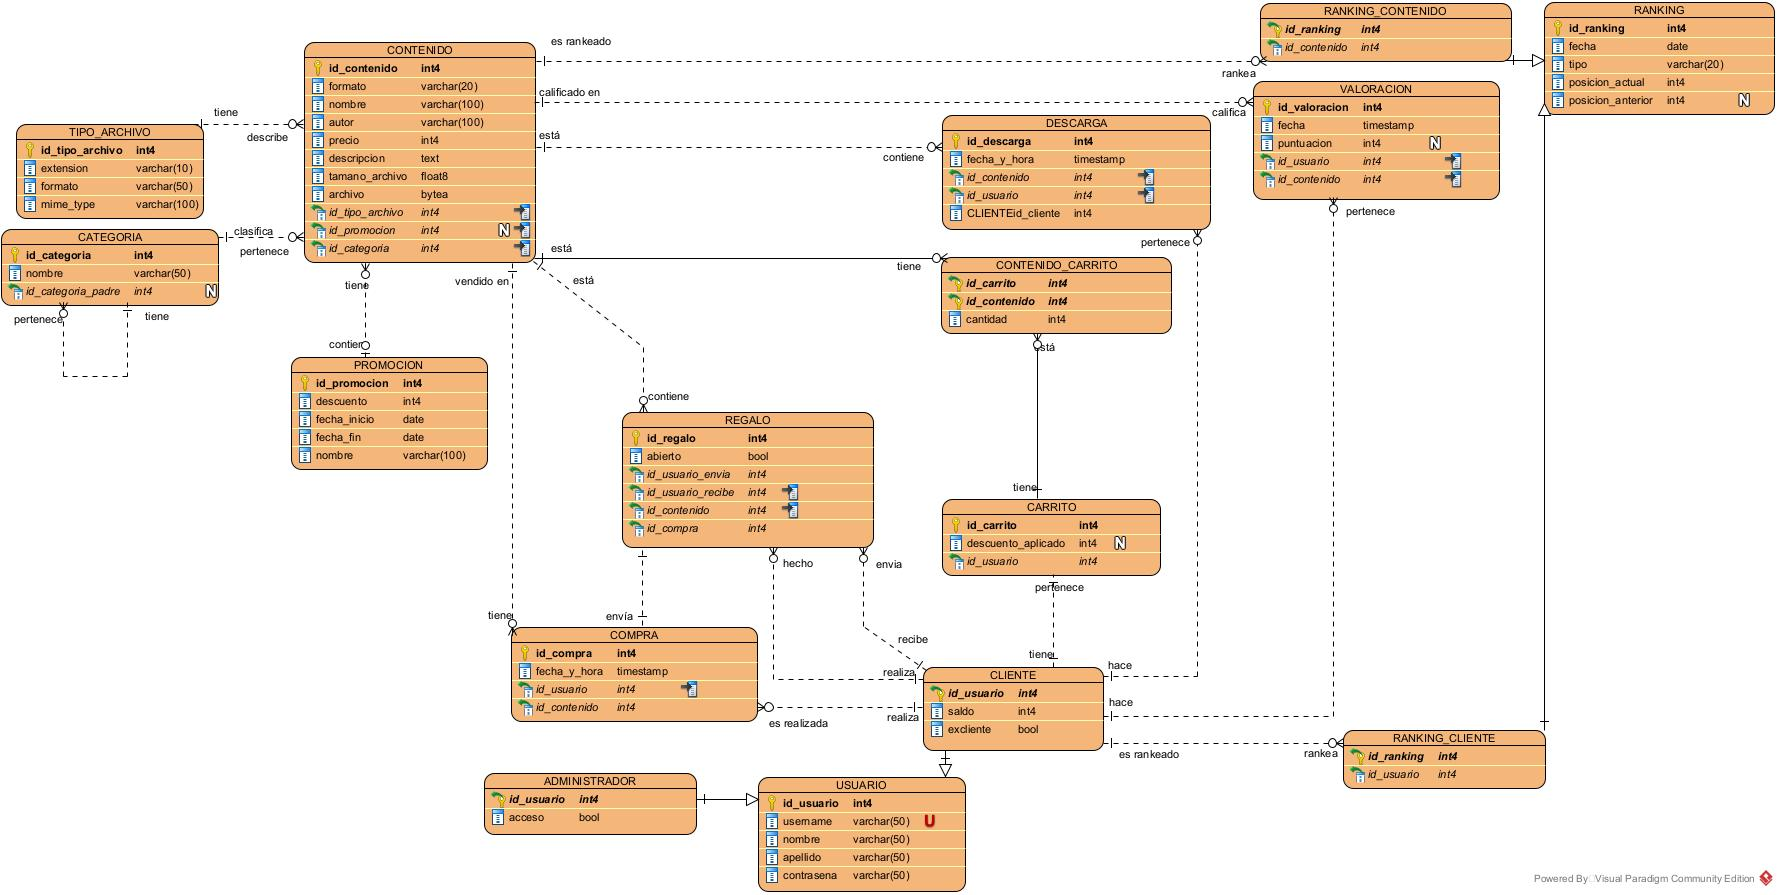
\includegraphics[width=0.9\textwidth]{Media/5_Desarrollo/MF.jpg}
    \caption{Diagrama del modelo físico (MF-001) del sistema QuickContentMedia} 
    \label{fig:DiagramaModeloFisico}
\end{figure}

\textbf{Archivo:} Diagrama del Modelo Físico (formato Visual Paradigm) \\
\textbf{Link de descarga:} \linkDiagramaModeloFisico \\
\newpage
\textbf{Pasos de ejecución:}
\begin{itemize}
    \item Ingresar al repositorio en GitHub usando el link proporcionado y descargar el archivo \texttt{QCM.vpp}.
    \item En la pestaña Database Modeling/Entity Relationship Model abrir el modelo físico.
\end{itemize}